\documentclass[conference,10pt]{IEEEtran}

\usepackage[T1]{fontenc}
\usepackage[utf8]{inputenc}
\usepackage[spanish,es-nodecimaldot,es-tabla]{babel}
\spanishplainpercent
\usepackage{amsmath,amssymb}
\usepackage{booktabs}
\usepackage{xcolor}
\usepackage{graphicx}
\usepackage[american]{circuitikz}
\usetikzlibrary{babel}

\graphicspath{{img/}}

% Tamaño de letra uniforme para todas las tablas
\usepackage{etoolbox}
\AtBeginEnvironment{table}{\footnotesize}
\AtBeginEnvironment{table*}{\footnotesize}

\title{Informe: Circuitos Resistivos - Parte 2\\
Práctica de Laboratorio No. 3}

\author{
  \IEEEauthorblockN{Maria Paula Mejía Vásquez, Cristian Alejandro Guarin Marin}
  \IEEEauthorblockA{
    Ingeniería Electrónica y de Telecomunicaciones\\
    Circuitos Eléctricos I -- Universidad de Antioquia\\
    Periodo 2026-2\\
    paula.mejia3@udea.edu.co, cristian.guarinm@udea.edu.co
  }
}

\begin{document}
\maketitle

\begin{abstract}
Este informe presenta el desarrollo de la Práctica de Laboratorio No. 3, en la que se verifican experimentalmente las Leyes de Kirchhoff de Corriente (LCK) y de Voltaje (LVK) sobre un circuito resistivo de dos mallas y cuatro nodos. A partir de los resultados teóricos del preinforme (análisis nodal y de mallas), se simula el circuito en LTspice y se realiza su montaje físico en protoboard, midiendo los voltajes de nodo y las corrientes de malla con la referencia de tierra en el nodo $d$ y, posteriormente, los voltajes de nodo con la referencia en el nodo $c$. La simulación reproduce el preinforme con diferencias menores a $1~\mathrm{mV}$, y la mayoría de las mediciones concuerda con la teoría una vez se consideran los valores reales de los resistores; se identifican y discuten dos lecturas atípicas ($v_c$ e $i_1$ con referencia en $d$). Se comprueba que los voltajes de nodo cambian al desplazar la referencia, mientras que los voltajes de los componentes permanecen invariantes.
\end{abstract}

\begin{IEEEkeywords}
Leyes de Kirchhoff, análisis nodal, análisis de mallas, circuitos resistivos, LTspice, protoboard.
\end{IEEEkeywords}

\section{Introducción}
El análisis sistemático de circuitos eléctricos requiere el dominio de herramientas matemáticas que permitan determinar voltajes y corrientes en cualquier punto de una red. Las Leyes de Kirchhoff, junto con la Ley de Ohm, constituyen el pilar de los métodos de análisis nodal (basado en la LCK) y de mallas (basado en la LVK) \cite{texto}. En el preinforme de esta práctica \cite{preinforme} se desarrollaron dichos análisis de forma teórica para un circuito de dos mallas y cuatro nodos, obteniendo los voltajes de nodo y las corrientes de malla con la referencia de tierra ubicada en el nodo $d$.

En este informe, siguiendo la guía de la práctica \cite{guia}, se contrastan esos resultados teóricos con la simulación del mismo circuito en LTspice y con su montaje físico en protoboard, empleando un multímetro para medir voltajes y corrientes. Adicionalmente, se repite la medición de los voltajes de nodo ubicando la referencia de tierra en el nodo $c$, con el fin de verificar que el valor de los voltajes de nodo depende de la referencia elegida, mientras que los voltajes de los componentes (diferencias entre dos nodos) no dependen de ella.

\section{Objetivos}
\subsection{Objetivo general}
Verificar experimentalmente, mediante simulación en LTspice y montaje físico en protoboard, el cumplimiento de las Leyes de Kirchhoff de corriente (LCK) y de voltaje (LVK) en un circuito resistivo de dos mallas, contrastando los resultados con los obtenidos teóricamente en el preinforme.

\subsection{Objetivos específicos}
\begin{itemize}
  \item Simular en LTspice el circuito propuesto y obtener los voltajes de nodo y las corrientes de los componentes mediante un análisis de punto de operación (.op).
  \item Realizar el montaje físico del circuito en protoboard y medir con el multímetro los voltajes de nodo y las corrientes de malla.
  \item Repetir la medición de los voltajes de nodo ubicando la referencia de tierra en el nodo $c$ y verificar que los voltajes de los componentes no cambian.
  \item Comparar los valores teóricos (preinforme), simulados y medidos, e identificar las causas de las diferencias encontradas.
  \item Verificar experimentalmente el cumplimiento de la LVK en cada malla y de la LCK en cada nodo a partir de los valores medidos.
\end{itemize}

\section{Materiales y medida de los resistores}
Para el desarrollo de la práctica se emplearon los siguientes materiales: protoboard, multímetro, fuente de voltaje dual ajustada a $v_1=8~\mathrm{V}$ y $v_2=6~\mathrm{V}$, cables de conexión y tres resistores comerciales seleccionados dentro del rango de $680~\Omega$ a $2.2~\mathrm{k}\Omega$ indicado por la guía: $R_1=680~\Omega$, $R_2=1000~\Omega$ y $R_3=2000~\Omega$, todos a $1/4~\mathrm{W}$ y con $1\,\%$ de tolerancia.

\begin{figure}[!htb]
  \centering
  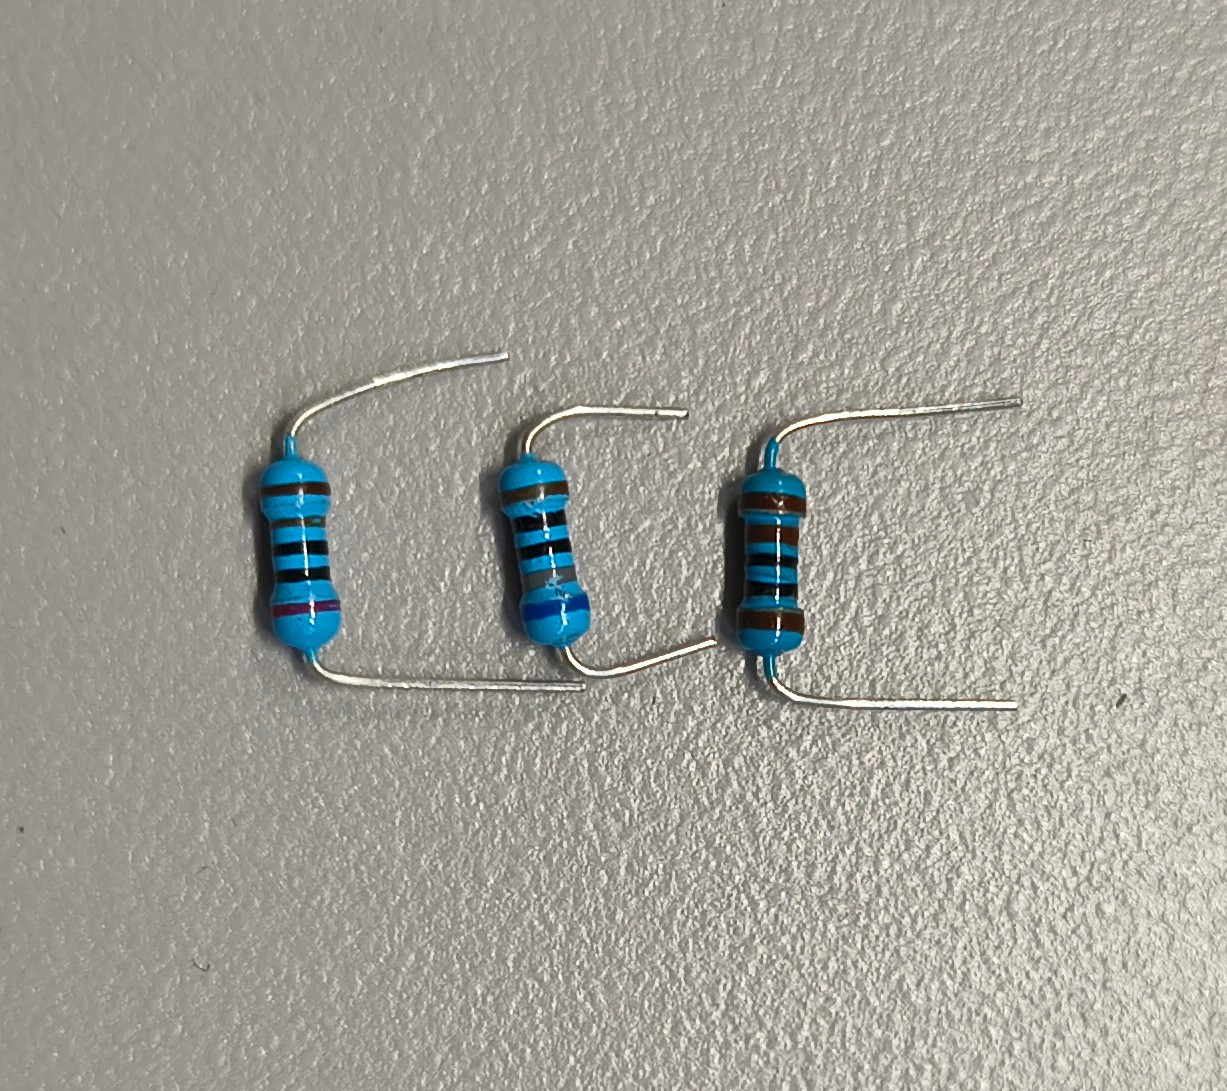
\includegraphics[width=0.8\linewidth]{resistores.jpg}
  \caption{Resistores $R_1$, $R_2$ y $R_3$ empleados en la práctica, donde se aprecia el código de colores de cada uno.}
  \label{fig:resistores}
\end{figure}

La Tabla~\ref{tab:medidas-resistencia} presenta el valor nominal de cada resistor, el rango de valores esperado según su código de colores ($\pm1\,\%$) y el valor medido con el multímetro antes del montaje del circuito.

\begin{table}[!htb]
  \caption{Valores medidos de resistencia}
  \label{tab:medidas-resistencia}
  \centering
  \begin{tabular}{ccccc}
    \toprule
    Resistor & Nominal & Rango esperado & Medido & Desviación \\
             & ($\Omega$) & ($\Omega$) & ($\Omega$) & \\
    \midrule
    $R_1$ & $680$  & $[673.2,\ 686.8]$ & $666$  & $-2.06\,\%$ \\
    $R_2$ & $1000$ & $[990,\ 1010]$    & $989$  & $-1.10\,\%$ \\
    $R_3$ & $2000$ & $[1980,\ 2020]$   & $1949$ & $-2.55\,\%$ \\
    \bottomrule
  \end{tabular}
\end{table}

Los tres resistores midieron levemente por debajo de su valor nominal y quedaron fuera de su banda de tolerancia: $R_1$ un $2.06\,\%$ por debajo ($7.2~\Omega$ bajo el límite inferior), $R_2$ un $1.10\,\%$ por debajo ($1~\Omega$ bajo el límite) y $R_3$ un $2.55\,\%$ por debajo ($31~\Omega$ bajo el límite). Las desviaciones son pequeñas y todas negativas, lo que puede deberse tanto al valor real de los componentes como a la exactitud del multímetro en la escala de resistencia. En la Sección~\ref{sec:comparacion} se muestra que, usando estos valores medidos en el cálculo teórico, se explica la mayor parte de las diferencias entre el preinforme y el montaje.

\section{Circuito bajo prueba}
El circuito analizado (Figura~\ref{fig:circuito-practica}) consta de dos fuentes de voltaje directo ($v_1=8~\mathrm{V}$, $v_2=6~\mathrm{V}$) y los tres resistores de la Tabla~\ref{tab:medidas-resistencia}, dispuestos en dos mallas que comparten la rama de $R_2$, con cuatro nodos identificados como $a$, $b$, $c$ y $d$. Las corrientes de malla $i_1$ e $i_2$ se definen en sentido horario.

\begin{figure}[!htb]
  \centering
  \begin{circuitikz}[american, scale=0.8, transform shape]
    \draw (0,0) -- (6,0);
    \draw (0,0) to[battery1, invert, l_=$v_1$, v^<=$8~\mathrm{V}$] (0,3) node[above] {$a$};
    \draw (0,3) to[R, l=$R_1$] (3,3) node[above] {$b$};
    \draw (3,3) to[R, l=$R_2$] (3,0);
    \draw (3,3) to[battery1, l=$v_2$, v_>=$6~\mathrm{V}$] (6,3) node[above] {$c$};
    \draw (6,3) to[R, l=$R_3$] (6,0);
    \draw (3,0) node[ground] {} node[above right] {$d$};
    \draw[->, red, thick] (1.0, 1.5) arc (180:-90:0.5);
    \node[red] at (1.5, 1.5) {$i_1$};
    \draw[->, red, thick] (4.0, 1.5) arc (180:-90:0.5);
    \node[red] at (4.5, 1.5) {$i_2$};
  \end{circuitikz}
  \caption{Circuito de la práctica, con referencia de tierra en el nodo $d$ y corrientes de malla en sentido horario.}
  \label{fig:circuito-practica}
\end{figure}

\section{Resultados teóricos (preinforme)}
\label{sec:preinforme}
En el preinforme \cite{preinforme} se desarrollaron el análisis nodal y el análisis de mallas del circuito de la Figura~\ref{fig:circuito-practica}, con valores nominales y la referencia de tierra en el nodo $d$ ($v_d=0~\mathrm{V}$). Los resultados obtenidos fueron:
\begin{align*}
  v_a &= 8.000~\mathrm{V}, & v_b &= 4.970~\mathrm{V},\\
  v_c &= -1.030~\mathrm{V}, & v_d &= 0~\mathrm{V},\\
  i_1 &= 4.455~\mathrm{mA}, & i_2 &= -0.5148~\mathrm{mA}.
\end{align*}
Estos valores se consignan en la fila \emph{Preinforme} de la Tabla~\ref{tab:ref-d}.

\section{Simulación (referencia en $d$)}
\label{sec:simulacion}
Se simuló el circuito en LTspice mediante un análisis de punto de operación (.op), con la tierra ubicada en el nodo $d$. La Figura~\ref{fig:sim-ref-d} muestra el esquemático y el resultado del análisis, donde $V(\mathrm{n001})=v_a$, $V(\mathrm{n002})=v_b$ y $V(\mathrm{n003})=v_c$.

\begin{figure}[!htb]
  \centering
  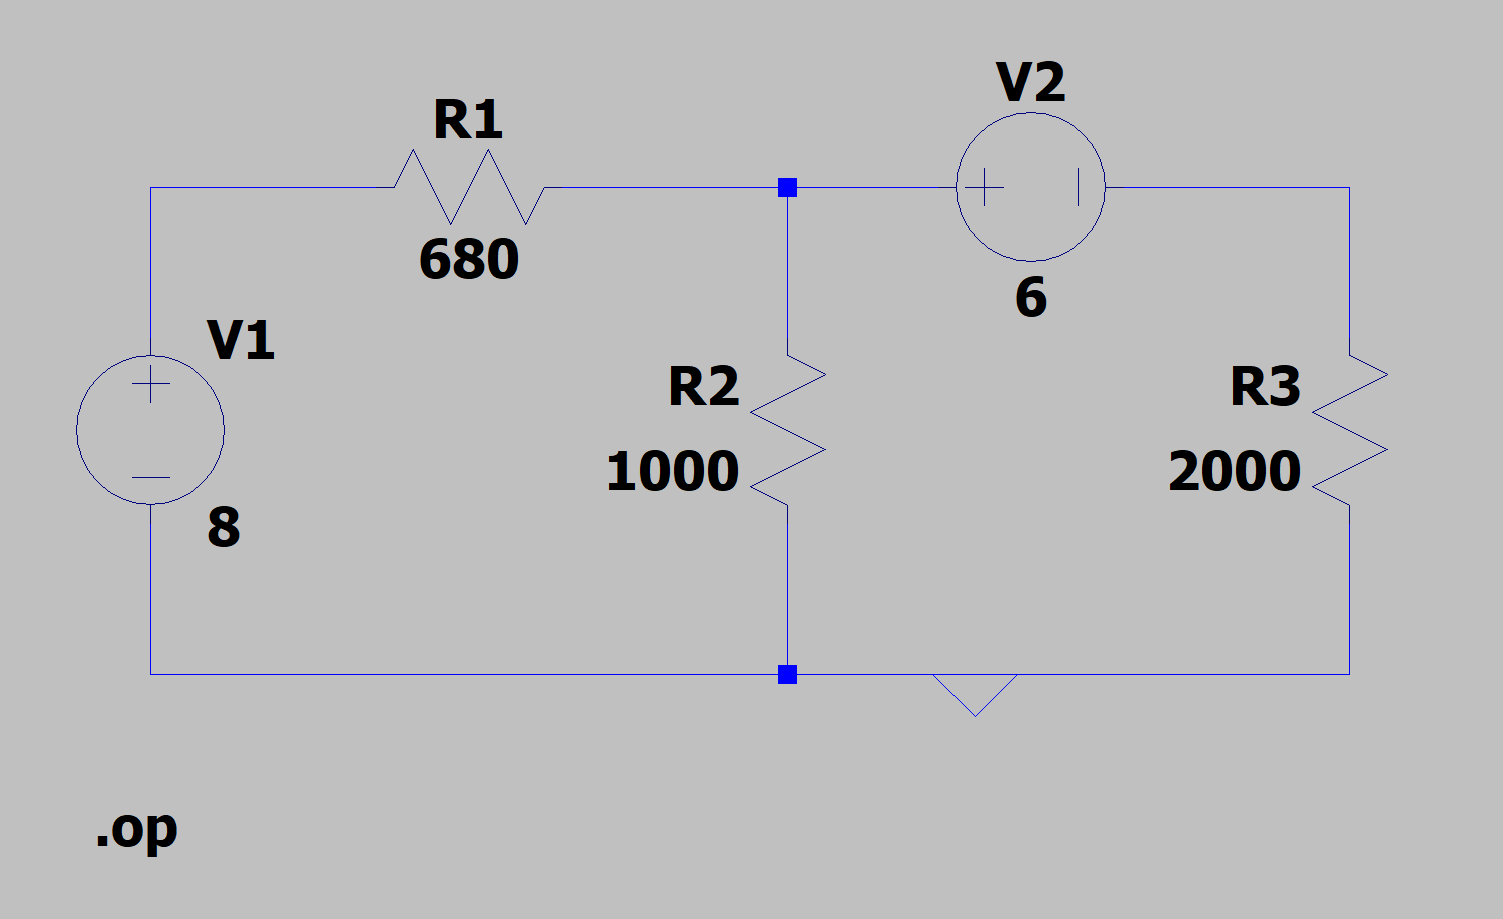
\includegraphics[width=0.9\linewidth]{esquematico_ref_d.png}\\[2pt]
  {\footnotesize (a)}\\[4pt]
  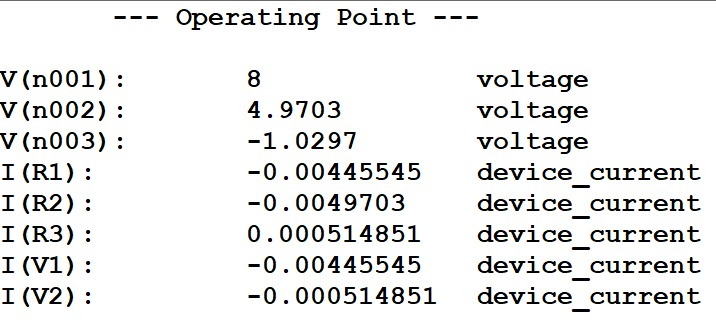
\includegraphics[width=0.9\linewidth]{operatingpoint_ref_d.jpg}\\[2pt]
  {\footnotesize (b)}
  \caption{Simulación en LTspice con la referencia en el nodo $d$: (a) esquemático; (b) resultado del análisis de punto de operación.}
  \label{fig:sim-ref-d}
\end{figure}

La simulación reporta $v_a=8~\mathrm{V}$, $v_b=4.9703~\mathrm{V}$ y $v_c=-1.0297~\mathrm{V}$, junto con las corrientes de todos los componentes: $I(R_1)=-4.45545~\mathrm{mA}$, $I(R_2)=-4.9703~\mathrm{mA}$, $I(R_3)=0.514851~\mathrm{mA}$, $I(V_1)=-4.45545~\mathrm{mA}$ e $I(V_2)=-0.514851~\mathrm{mA}$.

\subsection{Deducción de las corrientes de malla}
Cada corriente de malla es igual a la corriente de un componente que pertenezca \emph{únicamente} a esa malla; solo hay que tener en cuenta el sentido de referencia que LTspice usa para cada elemento. En una fuente de voltaje, LTspice reporta como positiva la corriente que entra por el terminal $+$ y recorre la fuente hasta el terminal $-$. Por lo tanto:
\begin{itemize}
  \item $V_1$ pertenece solo a la malla 1, e $i_1$ la recorre de $-$ a $+$ (de $d$ hacia $a$):
  \begin{equation*}
    i_1 = -I(V_1) = 4.455~\mathrm{mA}.
  \end{equation*}
  \item $V_2$ pertenece solo a la malla 2, e $i_2$ la recorre de $+$ a $-$ (de $b$ hacia $c$):
  \begin{equation*}
    i_2 = I(V_2) = -0.5149~\mathrm{mA}.
  \end{equation*}
\end{itemize}
El resultado es consistente con las demás corrientes: $|I(R_1)|=|i_1|$, $|I(R_3)|=|i_2|$ y en la rama compartida
\begin{equation*}
  |I(R_2)| = i_1 - i_2 = 4.455 + 0.515 = 4.970~\mathrm{mA}.
\end{equation*}
Estos valores se consignan en la fila \emph{Simulación} de la Tabla~\ref{tab:ref-d}.

\section{Montaje y medidas (referencia en $d$)}
\label{sec:montaje}
Se realizó el montaje del circuito de la Figura~\ref{fig:circuito-practica} en protoboard (Figura~\ref{fig:montaje}). Con el terminal común del multímetro en el nodo $d$ se midieron los voltajes de los nodos $a$, $b$ y $c$. Las corrientes de malla se obtuvieron midiendo la corriente en ramas que pertenecen a una sola malla ($R_1$ para $i_1$ y $R_3$ para $i_2$), expresadas con el sentido horario de la Figura~\ref{fig:circuito-practica}.

\begin{figure}[!htb]
  \centering
  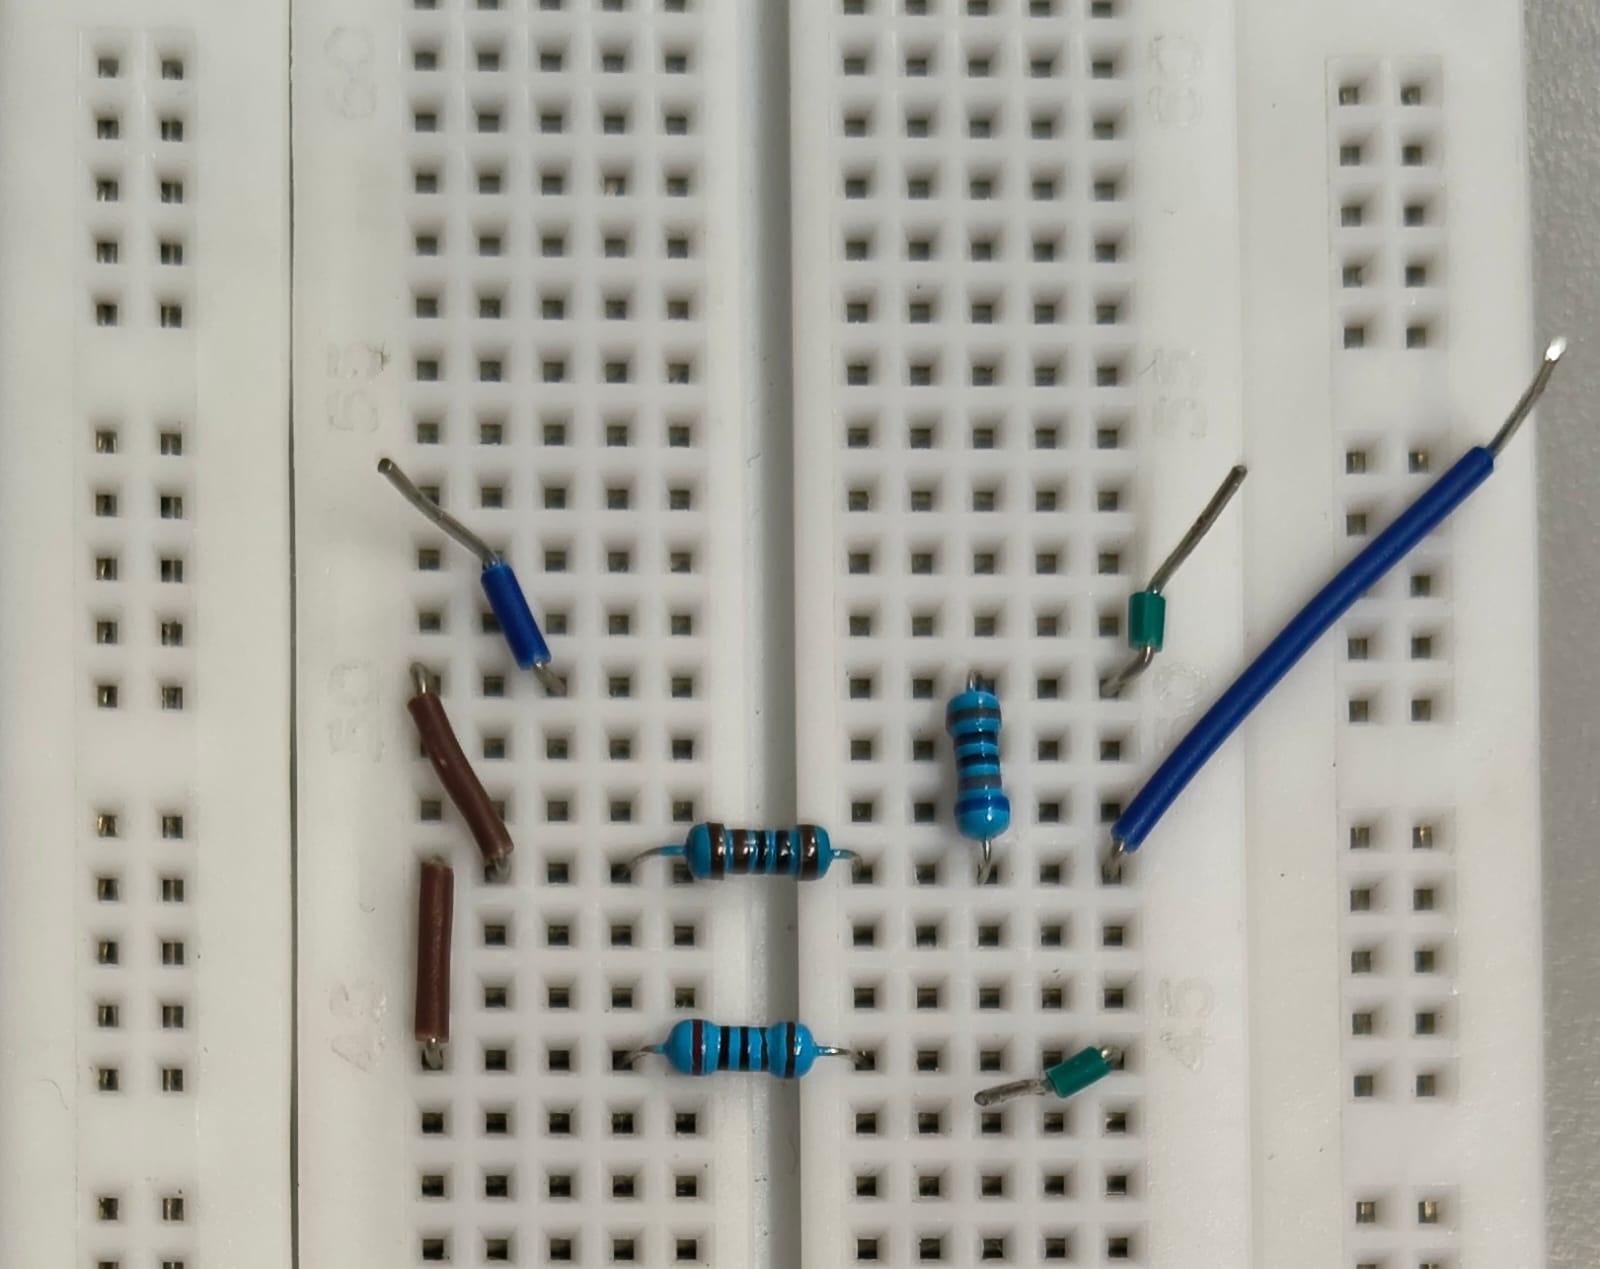
\includegraphics[width=0.8\linewidth]{montaje_practica3.jpg}
  \caption{Montaje físico del circuito de la Figura~\ref{fig:circuito-practica} en protoboard.}
  \label{fig:montaje}
\end{figure}

\begin{table}[!htb]
  \caption{Voltajes de nodo y corrientes de malla -- referencia nodo $d$}
  \label{tab:ref-d}
  \centering
  \setlength{\tabcolsep}{4pt}
  \begin{tabular}{lcccccc}
    \toprule
    & \multicolumn{4}{c}{Voltajes de nodo (V)} & \multicolumn{2}{c}{Corrientes de malla (mA)} \\
    \cmidrule(lr){2-5} \cmidrule(lr){6-7}
    & $v_a$ & $v_b$ & $v_c$ & $v_d$ & $i_1$ & $i_2$ \\
    \midrule
    Preinforme & $8.000$ & $4.970$  & $-1.030$  & $0$ & $4.455$  & $-0.5148$ \\
    Simulación & $8.000$ & $4.9703$ & $-1.0297$ & $0$ & $4.4554$ & $-0.5149$ \\
    Montaje    & $8.00$  & $4.99$   & $-0.69$   & $0$ & $4.82$   & $-0.51$ \\
    \bottomrule
  \end{tabular}
\end{table}

\subsection{Comparación de resultados}
\label{sec:comparacion}
\textbf{Preinforme frente a simulación.} Coinciden prácticamente de forma exacta: la mayor diferencia es de $0.3~\mathrm{mV}$ en voltajes y de $0.1~\mu\mathrm{A}$ en corrientes, atribuible solo al redondeo de los cálculos manuales. Esto confirma que el análisis nodal y de mallas del preinforme es correcto.

\textbf{Preinforme frente a montaje.} Para separar el efecto de los resistores reales, se repitió el análisis de mallas del preinforme usando los valores medidos de la Tabla~\ref{tab:medidas-resistencia} ($R_1=666~\Omega$, $R_2=989~\Omega$, $R_3=1949~\Omega$):
\begin{align*}
  i_1 &= 4.523~\mathrm{mA}, & i_2 &= -0.520~\mathrm{mA},\\
  v_b &= 4.987~\mathrm{V}, & v_c &= -1.013~\mathrm{V}.
\end{align*}
Con estos valores:
\begin{itemize}
  \item $v_a$, $v_b$ e $i_2$ medidos concuerdan con la teoría corregida con diferencias menores al $2\,\%$ ($4.99$ frente a $4.987~\mathrm{V}$; $-0.51$ frente a $-0.520~\mathrm{mA}$). Las diferencias restantes se deben a la resolución del multímetro y a su efecto de carga.
  \item $v_c=-0.69~\mathrm{V}$ se aleja un $32\,\%$ del valor esperado ($-1.013~\mathrm{V}$). Es una lectura atípica: la ley de Ohm con la corriente medida en $R_3$ da $v_{R3}=i_2R_3=-0.51\times1.949=-0.99~\mathrm{V}$, y la medición con referencia en $c$ (Sección~\ref{sec:ref-c}) da $v_c-v_d=-1.00~\mathrm{V}$. Además, implicaría que la fuente $v_2$ entrega $v_b-v_c=5.68~\mathrm{V}$, cuando con referencia en $c$ se midió directamente $5.99~\mathrm{V}$. Lo más probable es un mal contacto de la punta o una lectura en un punto distinto al nodo $c$.
  \item $i_1=4.82~\mathrm{mA}$ se aleja un $6.6\,\%$ del valor esperado ($4.523~\mathrm{mA}$). Tampoco se explica por la tolerancia de los resistores ni por la resistencia interna del amperímetro, que tendería a \emph{disminuir} la corriente. Por la ley de Ohm, $v_{R1}/R_1=3.01/666=4.52~\mathrm{mA}$, y al repetir la medición (Sección~\ref{sec:ref-c}) se obtuvo $4.51~\mathrm{mA}$; por tanto, la primera lectura se considera atípica.
\end{itemize}

En conclusión, los resultados del preinforme concuerdan con la simulación y, en general, con el montaje. Las diferencias sistemáticas se deben a que los resistores reales difieren de su valor nominal, y las dos desviaciones grandes ($v_c$ e $i_1$) corresponden a lecturas aisladas que no son consistentes con el resto de las mediciones.

\begin{table*}[!t]
  \caption{Voltajes de nodo con diferentes referencias (montaje, valores en V)}
  \label{tab:referencias}
  \centering
  \begin{tabular}{lccccccccc}
    \toprule
    & \multicolumn{4}{c}{Voltajes de nodo} & \multicolumn{5}{c}{Voltajes de los componentes} \\
    \cmidrule(lr){2-5} \cmidrule(lr){6-10}
    & $v_a$ & $v_b$ & $v_c$ & $v_d$ & $v_1$ & $v_2$ & $v_{R1}$ & $v_{R2}$ & $v_{R3}$ \\
    \midrule
    Referencia en nodo $d$ & $8.00$ & $4.99$ & $-0.69$ & $0$    & $8.00$ & $5.68$ & $3.01$ & $4.99$ & $-0.69$ \\
    Referencia en nodo $c$ & $9.00$ & $5.99$ & $0$     & $1.00$ & $8.00$ & $5.99$ & $3.01$ & $4.99$ & $-1.00$ \\
    \bottomrule
  \end{tabular}
\end{table*}

\section{Comprobación de las leyes de Kirchhoff}
\subsection{Ley de Voltajes de Kirchhoff}
A partir de los voltajes de nodo medidos con referencia en $d$ (Tabla~\ref{tab:ref-d}) se determinan los voltajes de los componentes de cada malla:
\begin{align*}
  v_1    &= v_a - v_d = 8.00 - 0 = 8.00~\mathrm{V},\\
  v_{R1} &= v_a - v_b = 8.00 - 4.99 = 3.01~\mathrm{V},\\
  v_{R2} &= v_b - v_d = 4.99 - 0 = 4.99~\mathrm{V},\\
  v_2    &= v_b - v_c = 4.99 - (-0.69) = 5.68~\mathrm{V},\\
  v_{R3} &= v_c - v_d = -0.69 - 0 = -0.69~\mathrm{V}.
\end{align*}

\textbf{Malla 1} (recorrido $a$--$b$--$d$--$a$ en el sentido de $i_1$):
\begin{equation*}
  -v_1 + v_{R1} + v_{R2} = -8.00 + 3.01 + 4.99 = 0.
\end{equation*}

\textbf{Malla 2} (recorrido $b$--$c$--$d$--$b$ en el sentido de $i_2$):
\begin{equation*}
  -v_{R2} + v_2 + v_{R3} = -4.99 + 5.68 - 0.69 = 0.
\end{equation*}

La suma de voltajes en cada malla es cero, por lo que se cumple la LVK. Como estos voltajes se obtienen a partir de voltajes de nodo, la suma siempre es cero. Por eso la lectura atípica de $v_c$ no altera la suma, pero sí se nota en el valor de $v_2$ ($5.68~\mathrm{V}$ en lugar de $6~\mathrm{V}$).

\subsection{Ley de Corrientes de Kirchhoff}
A partir de las corrientes de malla medidas ($i_1=4.82~\mathrm{mA}$, $i_2=-0.51~\mathrm{mA}$) se determinan las corrientes de rama:
\begin{align*}
  i_{R1} &= i_{v1} = i_1 = 4.82~\mathrm{mA} \quad (a\to b),\\
  i_{R2} &= i_1 - i_2 = 4.82 + 0.51 = 5.33~\mathrm{mA} \quad (b\to d),\\
  i_{R3} &= i_{v2} = i_2 = -0.51~\mathrm{mA} \quad (c\to d).
\end{align*}
Aplicando $\sum i_{\text{entra}} - \sum i_{\text{sale}} = 0$ en cada nodo:
\begin{align*}
  \text{Nodo } a&:\ i_{v1} - i_{R1} = 4.82 - 4.82 = 0,\\
  \text{Nodo } b&:\ i_{R1} - i_{R2} - i_{v2} = 4.82 - 5.33 + 0.51 = 0,\\
  \text{Nodo } c&:\ i_{v2} - i_{R3} = -0.51 + 0.51 = 0,\\
  \text{Nodo } d&:\ i_{R2} + i_{R3} - i_{v1} = 5.33 - 0.51 - 4.82 = 0.
\end{align*}
Al igual que con la LVK, esta comprobación se cumple siempre, porque las corrientes de rama se construyen con las corrientes de malla. Como verificación independiente, se calculan las corrientes de rama con la ley de Ohm a partir de los voltajes medidos, tomando $v_{R3}=-1.00~\mathrm{V}$ de la medición con referencia en $c$:
\begin{align*}
  i_{R1} &= 3.01/666 = 4.52~\mathrm{mA},\\
  i_{R2} &= 4.99/989 = 5.05~\mathrm{mA},\\
  i_{R3} &= -1.00/1949 = -0.51~\mathrm{mA}.
\end{align*}
En el supernodo $b$--$c$ se cumple
\begin{equation*}
  i_{R1} = i_{R2} + i_{R3}:\quad 4.52 \approx 5.05 - 0.51 = 4.54~\mathrm{mA},
\end{equation*}
con una diferencia del $0.4\,\%$, lo que confirma experimentalmente la LCK.

\section{Medidas con referencia en el nodo $c$}
\label{sec:ref-c}
Se trasladó el terminal común del multímetro al nodo $c$ y se midieron de nuevo los voltajes de nodo, obteniendo $v_a=9.00~\mathrm{V}$, $v_b=5.99~\mathrm{V}$ y $v_d=1.00~\mathrm{V}$. A partir de ellos se calculan los voltajes de los componentes:
\begin{align*}
  v_1    &= v_a - v_d = 9.00 - 1.00 = 8.00~\mathrm{V},\\
  v_{R1} &= v_a - v_b = 9.00 - 5.99 = 3.01~\mathrm{V},\\
  v_{R2} &= v_b - v_d = 5.99 - 1.00 = 4.99~\mathrm{V},\\
  v_2    &= v_b - v_c = 5.99 - 0 = 5.99~\mathrm{V},\\
  v_{R3} &= v_c - v_d = 0 - 1.00 = -1.00~\mathrm{V}.
\end{align*}
La Tabla~\ref{tab:referencias} reúne estos valores junto con los obtenidos con referencia en $d$.

Como verificación complementaria se simuló también el circuito con la tierra en el nodo $c$ (Figura~\ref{fig:sim-ref-c}). LTspice reporta $v_a=9.0297~\mathrm{V}$, $v_b=6~\mathrm{V}$ y $v_d=1.0297~\mathrm{V}$ (el nodo $c$ ya no aparece por ser la referencia, y el nodo $d$ se reporta como $V(\mathrm{n003})$), mientras que las corrientes de todos los componentes son idénticas a las de la Figura~\ref{fig:sim-ref-d}. En el montaje, al repetir la medición de corrientes con esta configuración se obtuvo $i_1=4.51~\mathrm{mA}$ e $i_2=-0.55~\mathrm{mA}$\footnote{En esta medición el multímetro se conectó con las puntas invertidas respecto a la de referencia en $d$; el valor ya está expresado en el sentido horario de la Figura~\ref{fig:circuito-practica}.}.

\begin{figure}[!htb]
  \centering
  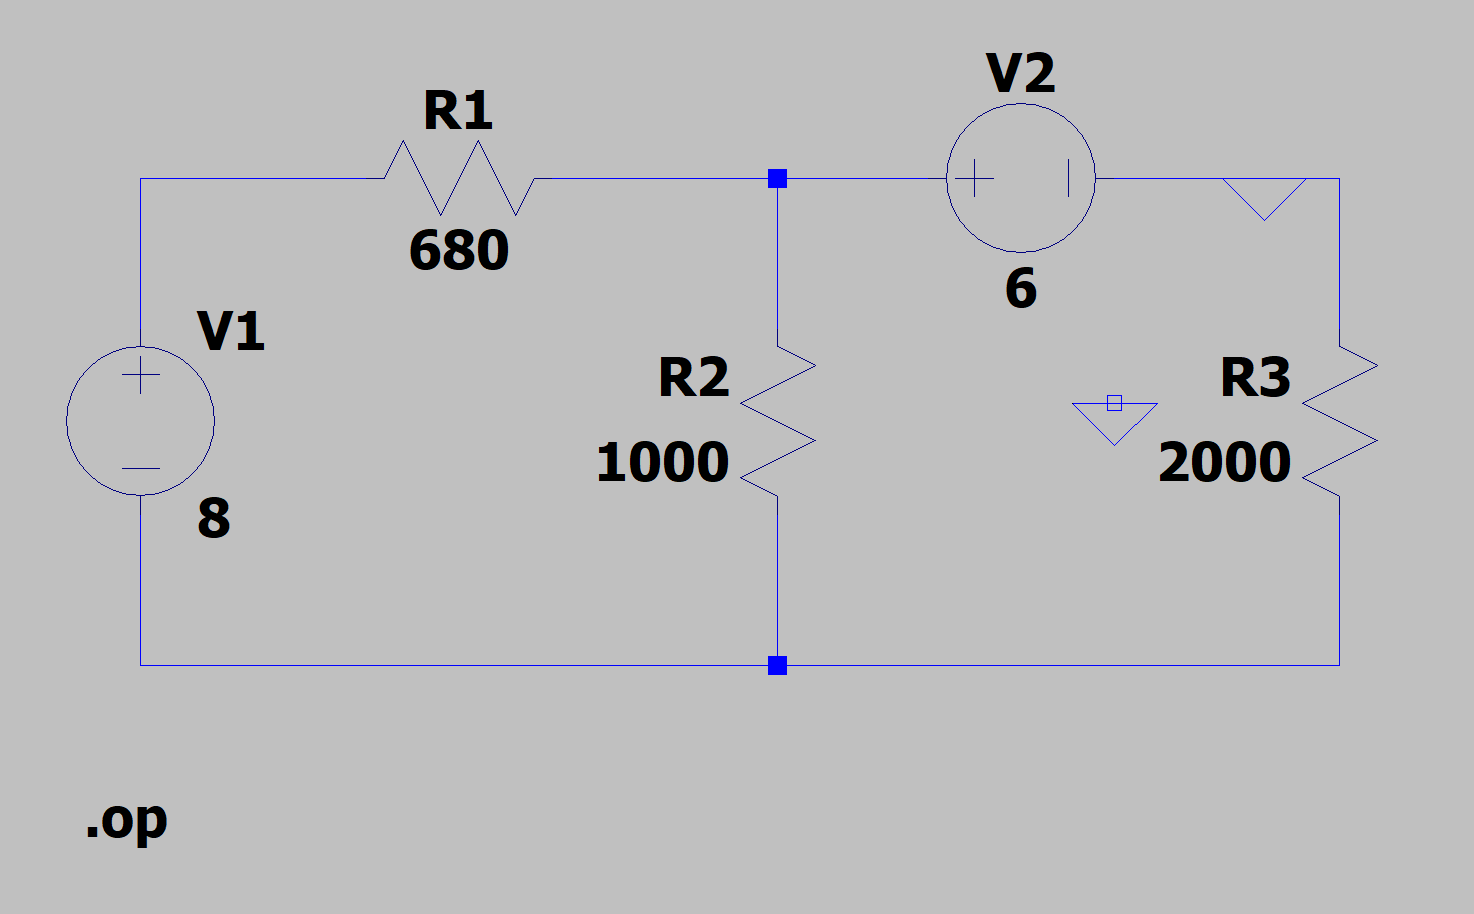
\includegraphics[width=0.9\linewidth]{esquematico_ref_c.png}\\[2pt]
  {\footnotesize (a)}\\[4pt]
  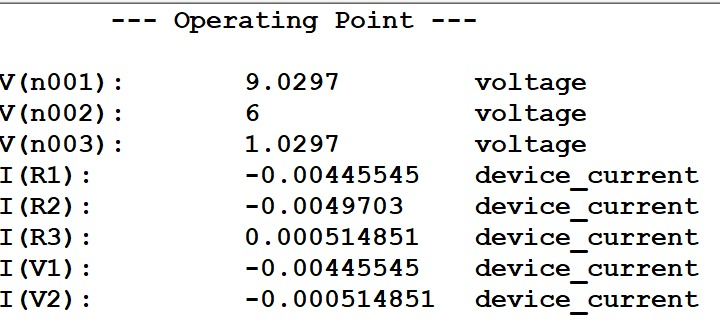
\includegraphics[width=0.9\linewidth]{operatingpoint_ref_c.jpg}\\[2pt]
  {\footnotesize (b)}
  \caption{Simulación en LTspice con la referencia en el nodo $c$: (a) esquemático; (b) resultado del análisis de punto de operación.}
  \label{fig:sim-ref-c}
\end{figure}

\subsection{Comparación entre referencias}
\begin{itemize}
  \item \textbf{Voltajes de nodo:} todos cambian al mover la referencia. Con la tierra en $c$, cada voltaje de nodo aumenta en la cantidad $-v_c$ (en simulación, exactamente $1.0297~\mathrm{V}$). Es decir, el voltaje de un nodo no es una magnitud absoluta, sino una diferencia de potencial respecto al nodo elegido como tierra.
  \item \textbf{Voltajes de los componentes:} $v_1$, $v_{R1}$ y $v_{R2}$ resultaron idénticos con ambas referencias ($8.00$, $3.01$ y $4.99~\mathrm{V}$), porque son diferencias entre dos nodos y el desplazamiento común se cancela.
  \item \textbf{Excepción:} $v_2$ y $v_{R3}$ difieren en $0.31~\mathrm{V}$ entre las dos filas de la Tabla~\ref{tab:referencias}. Esto no se debe al cambio de referencia, sino a la lectura atípica de $v_c$ con referencia en $d$ (Sección~\ref{sec:comparacion}). Los valores con referencia en $c$ ($5.99~\mathrm{V}$ y $-1.00~\mathrm{V}$) concuerdan con la fuente de $6~\mathrm{V}$ y con la teoría ($v_{R3}=-1.013~\mathrm{V}$ con resistores medidos).
\end{itemize}

\section{Conclusiones}
\textbf{Preinforme y simulación.} La simulación en LTspice reprodujo los voltajes de nodo y las corrientes de malla del preinforme con diferencias menores a $1~\mathrm{mV}$ y $1~\mu\mathrm{A}$, lo que valida el análisis nodal y de mallas realizado a mano. Las corrientes de malla se deducen de la simulación a partir de la corriente de un componente exclusivo de cada malla, teniendo en cuenta el sentido de referencia de LTspice.

\textbf{Montaje con referencia en $d$.} La mayoría de las mediciones concordó con la teoría. Las diferencias sistemáticas se explican por los valores reales de los resistores, que quedaron entre un $1.1\,\%$ y un $2.6\,\%$ por debajo de su valor nominal; al recalcular con ellos, $v_b$, $i_2$ e $i_1$ (en su segunda medición) coinciden con la teoría con diferencias menores al $2\,\%$. Las lecturas $v_c=-0.69~\mathrm{V}$ e $i_1=4.82~\mathrm{mA}$ son atípicas, por ser inconsistentes con la ley de Ohm y con las demás mediciones. Esto muestra la importancia de repetir y contrastar cada medida.

\textbf{Leyes de Kirchhoff.} La suma de voltajes en cada malla y la suma de corrientes en cada nodo fue cero con los datos medidos. La verificación independiente con la ley de Ohm en el supernodo $b$--$c$ cumplió la LCK con una diferencia del $0.4\,\%$.

\textbf{Cambio de referencia.} Al ubicar la tierra en el nodo $c$, todos los voltajes de nodo se desplazaron en una misma cantidad, mientras que los voltajes de los componentes ($v_1$, $v_{R1}$, $v_{R2}$) permanecieron iguales. La elección del nodo de referencia es arbitraria: solo cambia el valor numérico de los voltajes de nodo, no las diferencias de potencial ni las corrientes del circuito, que son las magnitudes físicas que describen las leyes de Kirchhoff.

\begin{thebibliography}{00}
  \bibitem{guia}
  Universidad de Antioquia, ``Guía de Práctica de Laboratorio: Circuitos Resistivos - Parte 2,'' Departamento de Ingeniería Electrónica y de Telecomunicaciones, Medellín, Colombia, 2026.
  \bibitem{preinforme}
  M. P. Mejía Vásquez y C. A. Guarín Marín, ``Preinforme: Circuitos Resistivos - Parte 2, Práctica de Laboratorio No. 3,'' Universidad de Antioquia, Medellín, Colombia, 2026.
  \bibitem{texto}
  C. K. Alexander y M. N. O. Sadiku, \emph{Fundamentos de circuitos eléctricos}, 5.ª ed. México D.F., México: McGraw-Hill Interamericana, 2013.
\end{thebibliography}

\end{document}
